% SPDX-License-Identifier: CC-BY-4.0
\documentclass{article}
\usepackage[margin=1in]{geometry}
\usepackage{graphicx} 
\usepackage[colorlinks=true, urlcolor=blue, linkcolor=red]{hyperref}

\begin{document}
\author{David Meeker}
\title{Alnico Magnet Properties}
\maketitle

\noindent Alnico magnet properties were gleaned from the following sources:

\begin{table}[htbp]
\centering
\begin{tabular}{|c|c|c|}
\hline
Grade & Demag Curve & Conductivity \\ \hline \hline
LNG10 & \href{https://web.archive.org/web/20230128141918/https://magnetsim.com/materials/cast-alnico}{IMI} &  \href{https://web.archive.org/web/20260323191135/https://www.arnoldmagnetics.com/wp-content/uploads/2017/10/Cast-Alnico-Permanent-Magnet-Brochure-101117.pdf}{Arnold} (Cast Alnico 3) 1.7 MS/m \\ \hline
LNG12 & \href{https://web.archive.org/web/20230128141918/https://magnetsim.com/materials/cast-alnico}{IMI} &  \href{https://web.archive.org/web/20260323191135/https://www.arnoldmagnetics.com/wp-content/uploads/2017/10/Cast-Alnico-Permanent-Magnet-Brochure-101117.pdf}{Arnold} (Cast Alnico 2) 1.5 MS/m \\ \hline
LNG37 & \href{https://web.archive.org/web/20230128141918/https://magnetsim.com/materials/cast-alnico}{IMI} &  \href{https://web.archive.org/web/20190325155903/http://www.magnetsales.com/Alnico/Alprops.htm}{Magnet Sales} (Cast Alnico 5) 2.1 MS/m \\ \hline
LNG40 & \href{https://web.archive.org/web/20230128141918/https://magnetsim.com/materials/cast-alnico}{IMI} (LNG37/LNG44 interpolation) &  \href{https://web.archive.org/web/20190325155903/http://www.magnetsales.com/Alnico/Alprops.htm}{Magnet Sales} (Cast Alnico 5) 2.1 MS/m \\ \hline
LNG44 & \href{https://web.archive.org/web/20230128141918/https://magnetsim.com/materials/cast-alnico}{IMI} &  \href{https://web.archive.org/web/20190325155903/http://www.magnetsales.com/Alnico/Alprops.htm}{Magnet Sales} (Cast Alnico 5) 2.1 MS/m \\ \hline
LNG56 & \href{https://web.archive.org/web/20230128141918/https://magnetsim.com/materials/cast-alnico}{IMI} &  \href{https://web.archive.org/web/20230629103524/https://cdn2.hubspot.net/hubfs/4788906/Electronenergy_December2018/Docs/EEC-Alnico-Material-Sheet.pdf}{EEC} (Cast Alnico 5-7) 2.1 MS/m \\ \hline
LNGT28 & \href{https://web.archive.org/web/20230128141918/https://magnetsim.com/materials/cast-alnico}{IMI} &  \href{https://web.archive.org/web/20230629103524/https://cdn2.hubspot.net/hubfs/4788906/Electronenergy_December2018/Docs/EEC-Alnico-Material-Sheet.pdf}{EEC} (Cast Alnico 6) 2 MS/m \\ \hline
LNGT32 & \href{https://web.archive.org/web/20230128141918/https://magnetsim.com/materials/cast-alnico}{IMI} &  \href{https://web.archive.org/web/20230629103524/https://cdn2.hubspot.net/hubfs/4788906/Electronenergy_December2018/Docs/EEC-Alnico-Material-Sheet.pdf}{EEC} (Cast Alnico 8) 1.9 MS/m \\ \hline
LNGT38 & \href{https://web.archive.org/web/20230128141918/https://magnetsim.com/materials/cast-alnico}{IMI} &  \href{https://web.archive.org/web/20230629103524/https://cdn2.hubspot.net/hubfs/4788906/Electronenergy_December2018/Docs/EEC-Alnico-Material-Sheet.pdf}{EEC} (Cast Alnico 8) 1.9 MS/m \\ \hline
LNGT44 & \href{https://web.archive.org/web/20230128141918/https://magnetsim.com/materials/cast-alnico}{IMI} &  \href{https://web.archive.org/web/20230629103524/https://cdn2.hubspot.net/hubfs/4788906/Electronenergy_December2018/Docs/EEC-Alnico-Material-Sheet.pdf}{EEC} (Cast Alnico 8) 1.9 MS/m \\ \hline
LNGT72 & \href{https://web.archive.org/web/20230128141918/https://magnetsim.com/materials/cast-alnico}{IMI} &  \href{https://web.archive.org/web/20230629103524/https://cdn2.hubspot.net/hubfs/4788906/Electronenergy_December2018/Docs/EEC-Alnico-Material-Sheet.pdf}{EEC} (Cast Alnico 9) 1.9 MS/m \\ \hline
FLNG12 & \href{https://web.archive.org/web/20230128123738/https://magnetsim.com/materials/sintered-alnico}{IMI} &  \href{https://web.archive.org/web/20230629103524/https://cdn2.hubspot.net/hubfs/4788906/Electronenergy_December2018/Docs/EEC-Alnico-Material-Sheet.pdf}{EEC} (Sintered Alnico 2) 1.5 MS/m \\ \hline
FLNG34 & \href{https://web.archive.org/web/20230128123738/https://magnetsim.com/materials/sintered-alnico}{IMI} &  \href{https://web.archive.org/web/20230629103524/https://cdn2.hubspot.net/hubfs/4788906/Electronenergy_December2018/Docs/EEC-Alnico-Material-Sheet.pdf}{EEC} (Sintered Alnico 5) 2 MS/m \\ \hline
FLNGT38 & \href{https://web.archive.org/web/20230128123738/https://magnetsim.com/materials/sintered-alnico}{IMI} (same as ``FLNG38'') &  \href{https://web.archive.org/web/20230629103524/https://cdn2.hubspot.net/hubfs/4788906/Electronenergy_December2018/Docs/EEC-Alnico-Material-Sheet.pdf}{EEC} (Sintered Alnico 8) 1.9 MS/m \\ \hline
\end{tabular}
\caption{Typical ALNICO properties}
\end{table}

\noindent To translate between various grade conventions, see \href{https://web.archive.org/web/20250806020511/https://allstarmagnetics.com/wp-content/uploads/2024/09/Alnico-Technical-Data-ASM.pdf}{this chart}.

\begin{figure} \centering
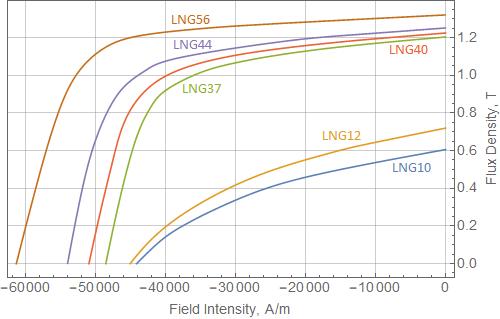
\includegraphics[height=3in]{alnicogroup1.png} \\
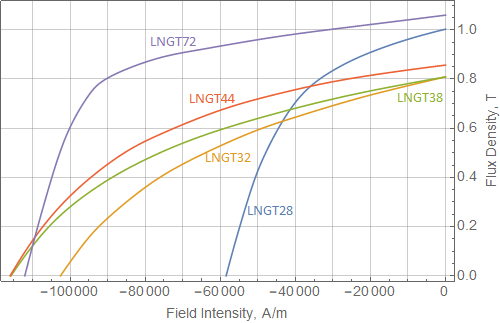
\includegraphics[height=3in]{alnicogroup2.png} \\
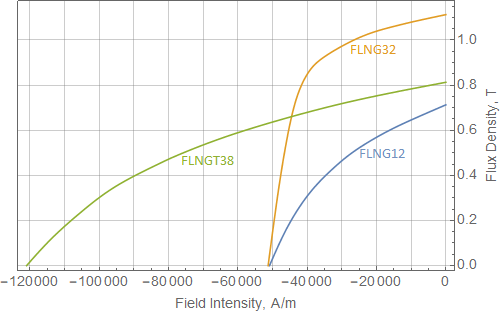
\includegraphics[height=3in]{alnicogroup3.png} \\
\caption{Plots of tabulated demagnetization curves}
\end{figure}

\noindent As a check, the IMI curves were compared with the typical demagnetization curves in Arnold's cast alnico brochure, which are drawn as vector artwork and so could be read exactly rather than traced. Where the grades correspond, the curves agree: LNG44 and Arnold's Alnico 5 are within 5~mT of each other out to 80\% of the coercivity, and LNG12 and Alnico 2 within 30~mT. Most of the other IMI curves lie 25--70~mT below Arnold's at 20\% of the coercivity, and further below near the knee. This is a difference of grade, not of reading: every IMI curve but one reproduces IMI's own tabulated remanence, coercivity and energy product for its grade to within about 6\% (the exception, FLNG12, has an energy product 14\% above its row, a row that is itself inconsistent, printing 1.4~kJ/m\(^3\) beside 1.55~MGOe), and each sits at the nominal energy product of its IEC grade (LNGT72 at 72~kJ/m\(^3\)), while Arnold quotes one typical value per grade, usually the higher one (83~kJ/m\(^3\) for Alnico 9). The IEC designations divide the old Alnico classes more finely; LNG37, LNG40 and LNG44 are all Alnico 5.

\noindent The pairing of LNG10 with Alnico 3 is the loosest in the table. The LNG10 curve agrees with IMI's own figures for the grade (0.60~T, 44~kA/m, 10~kJ/m\(^3\)), but LNG10 is not quite Alnico 3: Alnico 3 is the cobalt-free isotropic grade, with a higher remanence (0.70~T) and a lower coercivity (38~kA/m) at nearly the same energy product, and none of IMI's grades corresponds to it closely. The LNG10 entry is kept as the nearest available measured curve; its conductivity is Arnold's figure for Alnico 3.

\subsection*{References}
\noindent International Magnaproducts, \href{https://web.archive.org/web/20230128141918/https://magnetsim.com/materials/cast-alnico}{Cast Alnico}, accessed 28 Jan 2023. \\
\noindent International Magnaproducts, \href{https://web.archive.org/web/20230128123738/https://magnetsim.com/materials/sintered-alnico}{Sintered Alnico}, accessed 28 Jan 2023\\
\noindent Arnold Magnetics, \href{https://web.archive.org/web/20260323191135/https://www.arnoldmagnetics.com/wp-content/uploads/2017/10/Cast-Alnico-Permanent-Magnet-Brochure-101117.pdf}{Cast ALNICO Permanent Magnets}, accessed 23 Mar 2026. \\
\noindent Magnet Sales, \href{https://web.archive.org/web/20190325155903/http://www.magnetsales.com/Alnico/Alprops.htm}{Properties of Alnico Magnets}, accessed 25 Mar 2019. \\
\noindent Electron Energy Corporation, \href{https://web.archive.org/web/20230629103524/https://cdn2.hubspot.net/hubfs/4788906/Electronenergy_December2018/Docs/EEC-Alnico-Material-Sheet.pdf}{Alnico Magnets}, accessed 29 Jun 2023. \\
\noindent Allstar Magnetics, \href{https://web.archive.org/web/20250806020511/https://allstarmagnetics.com/wp-content/uploads/2024/09/Alnico-Technical-Data-ASM.pdf}{Magnetic Properties of Cast Alnico}, accessed 06 Aug 2025.

\noindent Copyright 2026 David Meeker. This document is licensed under the \href{https://creativecommons.org/licenses/by/4.0/}{Creative Commons Attribution 4.0 International License (CC BY 4.0)}.

\end{document}
